\section{Scratch}
\label{sec:scratch}

Scratch is chosen as the imperative language, and as the representative of the visual programming languages. As this causes the language to differ in both paradigm and writing style, it also affects the discussion on the criteria. Hence, there will be a focus on both aspects that differs from the other chosen languages.

\subsection{Iterator}
The iterator is made in a standard iterative way, through a simple loop. The debugging tool when clicking a piece of code is used to show a visual representation of the output in the game window. The control structure is a \emph{repeat} loop, which is the same as the well known \emph{for} loop, only with another name. The code for the program can be seen in \figref{fig:scratch_iter_code}, and the output is seen in \figref{fig:scratch_iter_out}.

\begin{figure}[h]
  \centering
    \begin{subfigure}[b]{0.45\textwidth}
    \begin{center}
      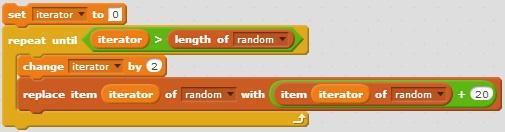
\includegraphics[scale=0.5]{./pics/scratch_iter_code}
      \caption{Scratch Iterator code.}
      \label{fig:scratch_iter_code}
    \end{center}
    \end{subfigure}
    ~
    \begin{subfigure}[b]{0.45\textwidth}
    \begin{center}
      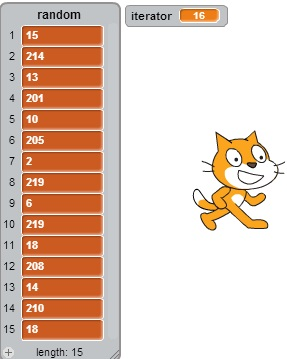
\includegraphics[scale=0.5]{./pics/scratch_iter_out}
      \caption{Scratch Iterator output.}
      \label{fig:scratch_iter_out}
    \end{center}
    \end{subfigure}
    \caption{Code and output for Hangman.}
    \label{fig:scratch_iter}
\end{figure}

\subsection{Fibonacci}
The fibonacci sequence is done through simple iteration in Scratch. The implementation can be seen in \figref{fig:scratch_fibo_code}. The user is asked to input how many numbers of the sequence are wanted. With a single loop and a selection, a list is presented, as seen in \figref{fig:scratch_fibo_out}.

\begin{figure}[h]
  \centering
    \begin{subfigure}[b]{0.45\textwidth}
    \begin{center}
      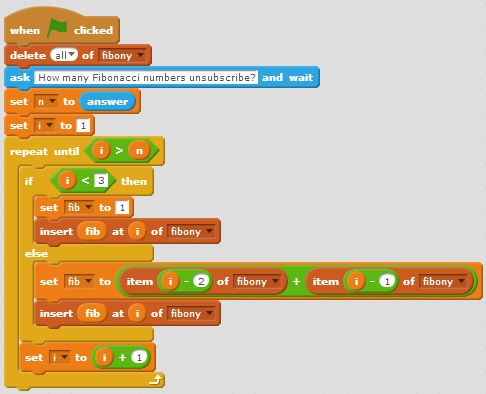
\includegraphics[scale=0.7]{./pics/scratch_fibo_code}
      \caption{Scratch fibonacci code.}
      \label{fig:scratch_fibo_code}
    \end{center}
    \end{subfigure}
    ~
    \begin{subfigure}[b]{0.45\textwidth}
    \begin{center}
      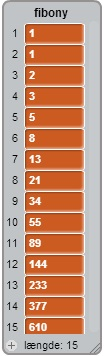
\includegraphics[scale=0.6]{./pics/scratch_fibo_out}
      \caption{Scratch fibonacci output.}
      \label{fig:scratch_fibo_out}
    \end{center}
    \end{subfigure}
    \caption{Code and output for fibonacci numbers.}
    \label{fig:scratch_fibo}
\end{figure}

\subsection{Cups and Ball}
The game of guessing the position of the ball amongst the cups is made with events, as Scratch is able to handle these with blocks. Events happen e.g. when a cup is clicked, cups are cloned, and when the ball is clicked. Code is also attached to different sprites, as these work individually to the events. The code blocks for the cups can be seen in \figref{fig:scratch_ball_code1}, and the code blocks for the ball can be seen in \figref{fig:scratch_ball_code2}. A screenshot of the game screen while in a game can be seen in \figref{fig:scratch_ball_out}.

\begin{figure}[h]
  \centering
    \begin{subfigure}[b]{0.45\textwidth}
    \begin{center}
      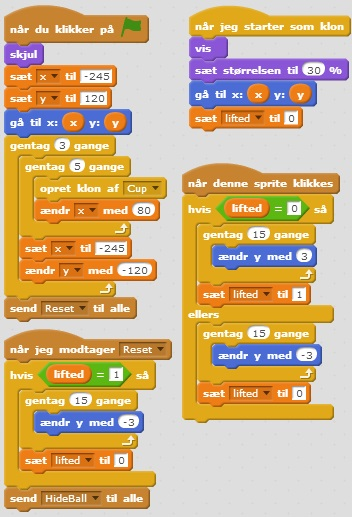
\includegraphics[scale=0.7]{./pics/scratch_ball_code1}
      \caption{Scratch cup code.}
      \label{fig:scratch_ball_code1}
    \end{center}
    \end{subfigure}
    ~
    \begin{subfigure}[b]{0.45\textwidth}
    \begin{center}
      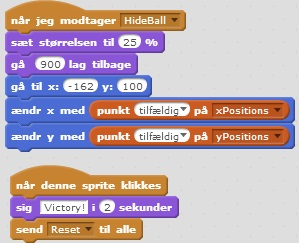
\includegraphics[scale=0.7]{./pics/scratch_ball_code2}
      \caption{Scratch ball code.}
      \label{fig:scratch_ball_code2}
    \end{center}
    \end{subfigure}
    
    \begin{subfigure}[b]{\textwidth}
    \begin{center}
      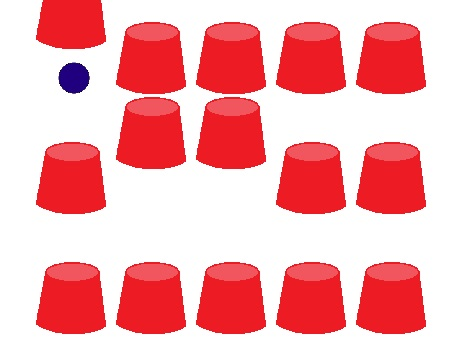
\includegraphics[scale=0.5]{./pics/scratch_ball_out}
      \caption{Scratch Cups and Ball output.}
      \label{fig:scratch_ball_out}
    \end{center}
    \end{subfigure}
    \caption{Code and output for Cups and Ball.}
    \label{fig:scratch_ball}
\end{figure}

\subsection{Hangman}
The Hangman game is made in an imperative manner. As there are many conditions to take into account, the code is rather long, and there is a lot of control structures. The guessing part itself is a big loop, which can be seen in \figref{fig:scratch_hang_code}. On the game screen, a list holds the letters for the word to guess, a list holds all the wrong guesses, and a sprite changes for each wrong guess. An input field is provided for guessing. The game screen can be seen in \figref{fig:scratch_hang_out}.

\begin{figure}[h]
  \centering
    \begin{subfigure}[b]{0.45\textwidth}
    \begin{center}
      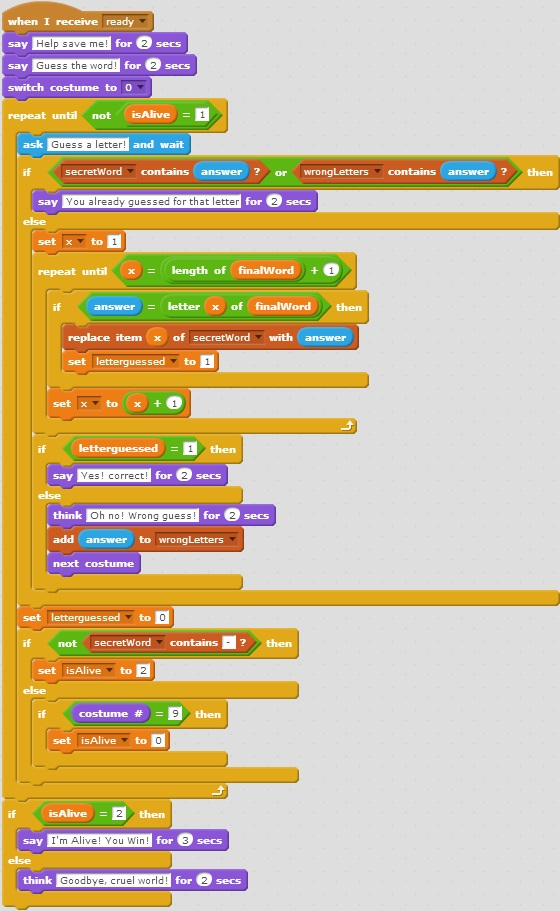
\includegraphics[scale=0.5]{./pics/scratch_hang_code}
      \caption{Scratch Hangman code.}
      \label{fig:scratch_hang_code}
    \end{center}
    \end{subfigure}
    ~
    \begin{subfigure}[b]{0.45\textwidth}
    \begin{center}
      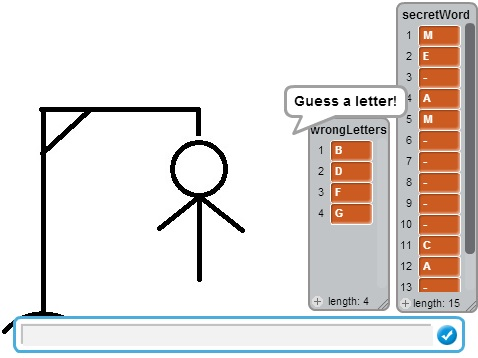
\includegraphics[scale=0.5]{./pics/scratch_hang_out}
      \caption{Scratch Hangman output.}
      \label{fig:scratch_hang_out}
    \end{center}
    \end{subfigure}
    \caption{Code and output for Hangman.}
    \label{fig:scratch_hang}
\end{figure}

\subsection{Criteria Evaluation}

\begin{description}[style=nextline]
\item[Readability] Scratch is known for its great readability, and this shows when reading it. The colored structures clearly show what the different building blocks are doing. The feature is unfortunately lost for color blind people, as it is not possible to change the colors. The language is very verbose in its statements and declarations, leading to a better understanding of what happens in a block. A problem lies in the fact that a project becomes very big very fast. An example of this can be seen in \figref{fig:scratch_hang_code}, where the collection of blocks seems hard to read at first glimpse, due to its sheer size.
\item[Writability] Scratch adds to better writability by providing categories with all its possible operations. It is easy to create simple structures, but it can get cumbersome if one has to write a lot of code. It is extremely easy to understand how to use Scratch, due to the fact that it uses building blocks as a way of constructing code.
\item[Observability] Scratch has a live game window, where output is shown when compiling code. Combined with the possibility of double-clicking sets of blocks to compile that specific piece of code, the programmer can see the effect whenever wanted.
\item[Trialability] The visual environment in Scratch allows no syntax errors. Combined with the level of observability, Scratch has great possibility of recovering from mistakes, as the mistake is easily found in the game window. In bigger programs, however, it can be hard to find the mistake, as one cannot follow the stack. Closing in on a small mistake that affects the whole program can be hard.
\item[Learnability] Making a game is a good way to capture the attention of children. But to keep them occupied, the process of coding should be intensive in a playful way. Building blocks from the visual style is a way to do it, as building blocks has been proven successful in the context of playing (Lego is an example of this).
\item[Reusability] As Scratch is also a minor game engine, it uses 2D sprites for visualization. Each sprite can contain code local to that sprite. The code shown in \figref{fig:scratch_ball_code1} is the code local to the Cup sprite, whereas the code shown in \figref{fig:scratch_ball_code2} is local to the Ball sprite. As these can be cloned, the code written serves as a blueprint for all instances of the sprite to use. However, the individual clone of a sprite cannot be accessed directly. Furthermore, Scratch has the possibility of defining custom blocks. These blocks can bring a collection of blocks down to the size of one, and they can easily be reused. These custom blocks work as functional procedures for the language.
\item[Pedagogic Value] Scratch makes use of the most basic of concepts, such as variables and control structures. That said, there is a huge leap when moving from Scratch to a non-visual programming language. The lack of conventional syntax, however, can be hindering further in the programmer's career. That means the language is great for novice programming, but it comes to a stop.
\item[Environment] Scratch has a very friendly environment, with great visibility in the color coding. As novices are not familiar with anything code-related, the naming of structures is meaningful and easy to understand. Navigation can be a bit confusing at first, as it can be hard to know what category a needed block is found in. The control of the blocks can be a bit annoying, as disconnecting interlocked blocks does not always go as expected. The game window combined with the block compilation, as mentioned, is a great way of obtaining feedback for trial-and-error.
\item[Documentation] Scratch has an integrated introduction tutorial, which is a great way for novices to learn the language. Furthermore, each building block can be right-clicked to find a documentation page for that specific block. This documentation is easy to read, but is unfortunately only available in English. Furthermore, it is possible to find and share projects via Scratch's homepage.
\item[Uniformity] The basic concepts used in Scratch do the same as in other languages. However, the naming of the expressions and structures are often different, e.g. Scratch has a \emph{repeat} structure, instead of a \emph{for} structure.
\item[Miscellaneous] Scratch uses sprites, but it is very hard to make different sprites work together, as the language itself is not object-oriented. As an example, you cannot reference to a specific sprite or one of its clones. Furthermore, the language has great accessibility in the fact that it is programmed in a browser.
\end{description}